% Created by tikzDevice version 0.12
% !TEX encoding = UTF-8 Unicode
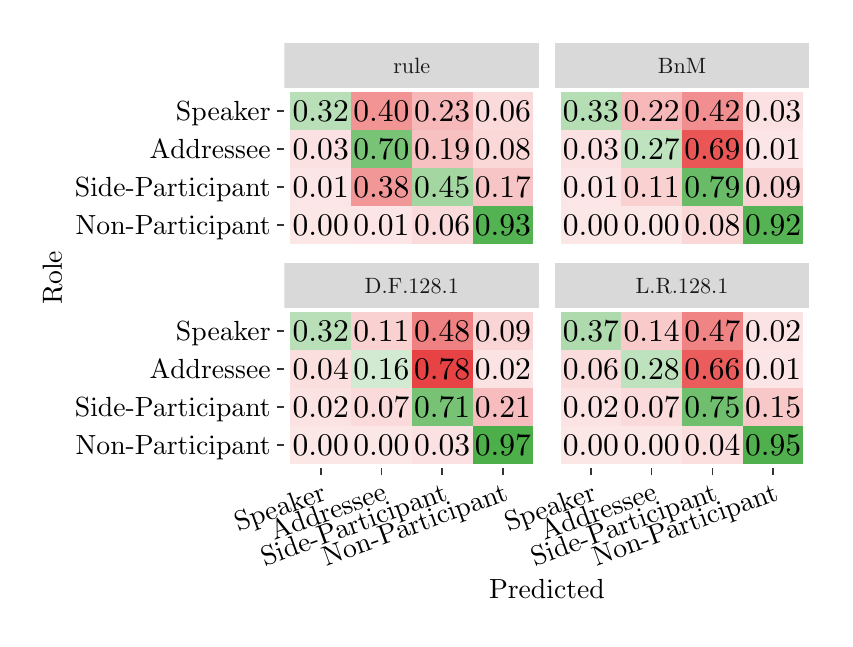
\begin{tikzpicture}[x=1pt,y=1pt]
\definecolor{fillColor}{RGB}{255,255,255}
\path[use as bounding box,fill=fillColor,fill opacity=0.00] (0,0) rectangle (288.00,213.58);
\begin{scope}
\path[clip] (  0.00,  0.00) rectangle (288.00,213.58);
\definecolor{drawColor}{RGB}{255,255,255}
\definecolor{fillColor}{RGB}{255,255,255}

\path[draw=drawColor,line width= 0.6pt,line join=round,line cap=round,fill=fillColor] (  0.00,  0.00) rectangle (288.00,213.58);
\end{scope}
\begin{scope}
\path[clip] ( 92.74,134.05) rectangle (184.87,191.83);
\definecolor{drawColor}{RGB}{255,255,255}

\path[draw=drawColor,line width= 0.6pt,line join=round] ( 92.74,142.30) --
	(184.87,142.30);

\path[draw=drawColor,line width= 0.6pt,line join=round] ( 92.74,156.06) --
	(184.87,156.06);

\path[draw=drawColor,line width= 0.6pt,line join=round] ( 92.74,169.82) --
	(184.87,169.82);

\path[draw=drawColor,line width= 0.6pt,line join=round] ( 92.74,183.57) --
	(184.87,183.57);

\path[draw=drawColor,line width= 0.6pt,line join=round] (105.90,134.05) --
	(105.90,191.83);

\path[draw=drawColor,line width= 0.6pt,line join=round] (127.83,134.05) --
	(127.83,191.83);

\path[draw=drawColor,line width= 0.6pt,line join=round] (149.77,134.05) --
	(149.77,191.83);

\path[draw=drawColor,line width= 0.6pt,line join=round] (171.71,134.05) --
	(171.71,191.83);
\definecolor{fillColor}{RGB}{77,175,74}

\path[fill=fillColor,fill opacity=0.39] ( 94.93,176.69) rectangle (116.87,190.45);
\definecolor{fillColor}{RGB}{228,26,28}

\path[fill=fillColor,fill opacity=0.47] (116.87,176.69) rectangle (138.80,190.45);
\definecolor{fillColor}{RGB}{228,26,28}

\path[fill=fillColor,fill opacity=0.31] (138.80,176.69) rectangle (160.74,190.45);
\definecolor{fillColor}{RGB}{228,26,28}

\path[fill=fillColor,fill opacity=0.16] (160.74,176.69) rectangle (182.67,190.45);
\definecolor{fillColor}{RGB}{228,26,28}

\path[fill=fillColor,fill opacity=0.13] ( 94.93,162.94) rectangle (116.87,176.69);
\definecolor{fillColor}{RGB}{77,175,74}

\path[fill=fillColor,fill opacity=0.75] (116.87,162.94) rectangle (138.80,176.69);
\definecolor{fillColor}{RGB}{228,26,28}

\path[fill=fillColor,fill opacity=0.27] (138.80,162.94) rectangle (160.74,176.69);
\definecolor{fillColor}{RGB}{228,26,28}

\path[fill=fillColor,fill opacity=0.17] (160.74,162.94) rectangle (182.67,176.69);
\definecolor{fillColor}{RGB}{228,26,28}

\path[fill=fillColor,fill opacity=0.11] ( 94.93,149.18) rectangle (116.87,162.94);
\definecolor{fillColor}{RGB}{228,26,28}

\path[fill=fillColor,fill opacity=0.45] (116.87,149.18) rectangle (138.80,162.94);
\definecolor{fillColor}{RGB}{77,175,74}

\path[fill=fillColor,fill opacity=0.51] (138.80,149.18) rectangle (160.74,162.94);
\definecolor{fillColor}{RGB}{228,26,28}

\path[fill=fillColor,fill opacity=0.25] (160.74,149.18) rectangle (182.67,162.94);
\definecolor{fillColor}{RGB}{228,26,28}

\path[fill=fillColor,fill opacity=0.10] ( 94.93,135.42) rectangle (116.87,149.18);
\definecolor{fillColor}{RGB}{228,26,28}

\path[fill=fillColor,fill opacity=0.11] (116.87,135.42) rectangle (138.80,149.18);
\definecolor{fillColor}{RGB}{228,26,28}

\path[fill=fillColor,fill opacity=0.16] (138.80,135.42) rectangle (160.74,149.18);
\definecolor{fillColor}{RGB}{77,175,74}

\path[fill=fillColor,fill opacity=0.96] (160.74,135.42) rectangle (182.67,149.18);
\definecolor{drawColor}{RGB}{0,0,0}

\node[text=drawColor,anchor=base,inner sep=0pt, outer sep=0pt, scale=  1.14] at (105.90,179.65) {0.32};

\node[text=drawColor,anchor=base,inner sep=0pt, outer sep=0pt, scale=  1.14] at (127.83,179.65) {0.40};

\node[text=drawColor,anchor=base,inner sep=0pt, outer sep=0pt, scale=  1.14] at (149.77,179.65) {0.23};

\node[text=drawColor,anchor=base,inner sep=0pt, outer sep=0pt, scale=  1.14] at (171.71,179.65) {0.06};

\node[text=drawColor,anchor=base,inner sep=0pt, outer sep=0pt, scale=  1.14] at (105.90,165.90) {0.03};

\node[text=drawColor,anchor=base,inner sep=0pt, outer sep=0pt, scale=  1.14] at (127.83,165.90) {0.70};

\node[text=drawColor,anchor=base,inner sep=0pt, outer sep=0pt, scale=  1.14] at (149.77,165.90) {0.19};

\node[text=drawColor,anchor=base,inner sep=0pt, outer sep=0pt, scale=  1.14] at (171.71,165.90) {0.08};

\node[text=drawColor,anchor=base,inner sep=0pt, outer sep=0pt, scale=  1.14] at (105.90,152.14) {0.01};

\node[text=drawColor,anchor=base,inner sep=0pt, outer sep=0pt, scale=  1.14] at (127.83,152.14) {0.38};

\node[text=drawColor,anchor=base,inner sep=0pt, outer sep=0pt, scale=  1.14] at (149.77,152.14) {0.45};

\node[text=drawColor,anchor=base,inner sep=0pt, outer sep=0pt, scale=  1.14] at (171.71,152.14) {0.17};

\node[text=drawColor,anchor=base,inner sep=0pt, outer sep=0pt, scale=  1.14] at (105.90,138.38) {0.00};

\node[text=drawColor,anchor=base,inner sep=0pt, outer sep=0pt, scale=  1.14] at (127.83,138.38) {0.01};

\node[text=drawColor,anchor=base,inner sep=0pt, outer sep=0pt, scale=  1.14] at (149.77,138.38) {0.06};

\node[text=drawColor,anchor=base,inner sep=0pt, outer sep=0pt, scale=  1.14] at (171.71,138.38) {0.93};
\end{scope}
\begin{scope}
\path[clip] ( 92.74, 54.51) rectangle (184.87,112.29);
\definecolor{drawColor}{RGB}{255,255,255}

\path[draw=drawColor,line width= 0.6pt,line join=round] ( 92.74, 62.77) --
	(184.87, 62.77);

\path[draw=drawColor,line width= 0.6pt,line join=round] ( 92.74, 76.52) --
	(184.87, 76.52);

\path[draw=drawColor,line width= 0.6pt,line join=round] ( 92.74, 90.28) --
	(184.87, 90.28);

\path[draw=drawColor,line width= 0.6pt,line join=round] ( 92.74,104.04) --
	(184.87,104.04);

\path[draw=drawColor,line width= 0.6pt,line join=round] (105.90, 54.51) --
	(105.90,112.29);

\path[draw=drawColor,line width= 0.6pt,line join=round] (127.83, 54.51) --
	(127.83,112.29);

\path[draw=drawColor,line width= 0.6pt,line join=round] (149.77, 54.51) --
	(149.77,112.29);

\path[draw=drawColor,line width= 0.6pt,line join=round] (171.71, 54.51) --
	(171.71,112.29);
\definecolor{fillColor}{RGB}{77,175,74}

\path[fill=fillColor,fill opacity=0.39] ( 94.93, 97.16) rectangle (116.87,110.92);
\definecolor{fillColor}{RGB}{228,26,28}

\path[fill=fillColor,fill opacity=0.20] (116.87, 97.16) rectangle (138.80,110.92);
\definecolor{fillColor}{RGB}{228,26,28}

\path[fill=fillColor,fill opacity=0.55] (138.80, 97.16) rectangle (160.74,110.92);
\definecolor{fillColor}{RGB}{228,26,28}

\path[fill=fillColor,fill opacity=0.18] (160.74, 97.16) rectangle (182.67,110.92);
\definecolor{fillColor}{RGB}{228,26,28}

\path[fill=fillColor,fill opacity=0.14] ( 94.93, 83.40) rectangle (116.87, 97.16);
\definecolor{fillColor}{RGB}{77,175,74}

\path[fill=fillColor,fill opacity=0.25] (116.87, 83.40) rectangle (138.80, 97.16);
\definecolor{fillColor}{RGB}{228,26,28}

\path[fill=fillColor,fill opacity=0.82] (138.80, 83.40) rectangle (160.74, 97.16);
\definecolor{fillColor}{RGB}{228,26,28}

\path[fill=fillColor,fill opacity=0.12] (160.74, 83.40) rectangle (182.67, 97.16);
\definecolor{fillColor}{RGB}{228,26,28}

\path[fill=fillColor,fill opacity=0.12] ( 94.93, 69.65) rectangle (116.87, 83.40);
\definecolor{fillColor}{RGB}{228,26,28}

\path[fill=fillColor,fill opacity=0.16] (116.87, 69.65) rectangle (138.80, 83.40);
\definecolor{fillColor}{RGB}{77,175,74}

\path[fill=fillColor,fill opacity=0.76] (138.80, 69.65) rectangle (160.74, 83.40);
\definecolor{fillColor}{RGB}{228,26,28}

\path[fill=fillColor,fill opacity=0.29] (160.74, 69.65) rectangle (182.67, 83.40);
\definecolor{fillColor}{RGB}{228,26,28}

\path[fill=fillColor,fill opacity=0.10] ( 94.93, 55.89) rectangle (116.87, 69.65);

\path[fill=fillColor,fill opacity=0.10] (116.87, 55.89) rectangle (138.80, 69.65);
\definecolor{fillColor}{RGB}{228,26,28}

\path[fill=fillColor,fill opacity=0.13] (138.80, 55.89) rectangle (160.74, 69.65);
\definecolor{fillColor}{RGB}{77,175,74}

\path[fill=fillColor] (160.74, 55.89) rectangle (182.67, 69.65);
\definecolor{drawColor}{RGB}{0,0,0}

\node[text=drawColor,anchor=base,inner sep=0pt, outer sep=0pt, scale=  1.14] at (105.90,100.12) {0.32};

\node[text=drawColor,anchor=base,inner sep=0pt, outer sep=0pt, scale=  1.14] at (127.83,100.12) {0.11};

\node[text=drawColor,anchor=base,inner sep=0pt, outer sep=0pt, scale=  1.14] at (149.77,100.12) {0.48};

\node[text=drawColor,anchor=base,inner sep=0pt, outer sep=0pt, scale=  1.14] at (171.71,100.12) {0.09};

\node[text=drawColor,anchor=base,inner sep=0pt, outer sep=0pt, scale=  1.14] at (105.90, 86.36) {0.04};

\node[text=drawColor,anchor=base,inner sep=0pt, outer sep=0pt, scale=  1.14] at (127.83, 86.36) {0.16};

\node[text=drawColor,anchor=base,inner sep=0pt, outer sep=0pt, scale=  1.14] at (149.77, 86.36) {0.78};

\node[text=drawColor,anchor=base,inner sep=0pt, outer sep=0pt, scale=  1.14] at (171.71, 86.36) {0.02};

\node[text=drawColor,anchor=base,inner sep=0pt, outer sep=0pt, scale=  1.14] at (105.90, 72.61) {0.02};

\node[text=drawColor,anchor=base,inner sep=0pt, outer sep=0pt, scale=  1.14] at (127.83, 72.61) {0.07};

\node[text=drawColor,anchor=base,inner sep=0pt, outer sep=0pt, scale=  1.14] at (149.77, 72.61) {0.71};

\node[text=drawColor,anchor=base,inner sep=0pt, outer sep=0pt, scale=  1.14] at (171.71, 72.61) {0.21};

\node[text=drawColor,anchor=base,inner sep=0pt, outer sep=0pt, scale=  1.14] at (105.90, 58.85) {0.00};

\node[text=drawColor,anchor=base,inner sep=0pt, outer sep=0pt, scale=  1.14] at (127.83, 58.85) {0.00};

\node[text=drawColor,anchor=base,inner sep=0pt, outer sep=0pt, scale=  1.14] at (149.77, 58.85) {0.03};

\node[text=drawColor,anchor=base,inner sep=0pt, outer sep=0pt, scale=  1.14] at (171.71, 58.85) {0.97};
\end{scope}
\begin{scope}
\path[clip] (190.37,134.05) rectangle (282.50,191.83);
\definecolor{drawColor}{RGB}{255,255,255}

\path[draw=drawColor,line width= 0.6pt,line join=round] (190.37,142.30) --
	(282.50,142.30);

\path[draw=drawColor,line width= 0.6pt,line join=round] (190.37,156.06) --
	(282.50,156.06);

\path[draw=drawColor,line width= 0.6pt,line join=round] (190.37,169.82) --
	(282.50,169.82);

\path[draw=drawColor,line width= 0.6pt,line join=round] (190.37,183.57) --
	(282.50,183.57);

\path[draw=drawColor,line width= 0.6pt,line join=round] (203.53,134.05) --
	(203.53,191.83);

\path[draw=drawColor,line width= 0.6pt,line join=round] (225.47,134.05) --
	(225.47,191.83);

\path[draw=drawColor,line width= 0.6pt,line join=round] (247.40,134.05) --
	(247.40,191.83);

\path[draw=drawColor,line width= 0.6pt,line join=round] (269.34,134.05) --
	(269.34,191.83);
\definecolor{fillColor}{RGB}{77,175,74}

\path[fill=fillColor,fill opacity=0.41] (192.56,176.69) rectangle (214.50,190.45);
\definecolor{fillColor}{RGB}{228,26,28}

\path[fill=fillColor,fill opacity=0.31] (214.50,176.69) rectangle (236.43,190.45);
\definecolor{fillColor}{RGB}{228,26,28}

\path[fill=fillColor,fill opacity=0.49] (236.43,176.69) rectangle (258.37,190.45);
\definecolor{fillColor}{RGB}{228,26,28}

\path[fill=fillColor,fill opacity=0.13] (258.37,176.69) rectangle (280.31,190.45);
\definecolor{fillColor}{RGB}{228,26,28}

\path[fill=fillColor,fill opacity=0.13] (192.56,162.94) rectangle (214.50,176.69);
\definecolor{fillColor}{RGB}{77,175,74}

\path[fill=fillColor,fill opacity=0.35] (214.50,162.94) rectangle (236.43,176.69);
\definecolor{fillColor}{RGB}{228,26,28}

\path[fill=fillColor,fill opacity=0.74] (236.43,162.94) rectangle (258.37,176.69);
\definecolor{fillColor}{RGB}{228,26,28}

\path[fill=fillColor,fill opacity=0.11] (258.37,162.94) rectangle (280.31,176.69);
\definecolor{fillColor}{RGB}{228,26,28}

\path[fill=fillColor,fill opacity=0.11] (192.56,149.18) rectangle (214.50,162.94);
\definecolor{fillColor}{RGB}{228,26,28}

\path[fill=fillColor,fill opacity=0.20] (214.50,149.18) rectangle (236.43,162.94);
\definecolor{fillColor}{RGB}{77,175,74}

\path[fill=fillColor,fill opacity=0.84] (236.43,149.18) rectangle (258.37,162.94);
\definecolor{fillColor}{RGB}{228,26,28}

\path[fill=fillColor,fill opacity=0.19] (258.37,149.18) rectangle (280.31,162.94);
\definecolor{fillColor}{RGB}{228,26,28}

\path[fill=fillColor,fill opacity=0.10] (192.56,135.42) rectangle (214.50,149.18);

\path[fill=fillColor,fill opacity=0.10] (214.50,135.42) rectangle (236.43,149.18);
\definecolor{fillColor}{RGB}{228,26,28}

\path[fill=fillColor,fill opacity=0.17] (236.43,135.42) rectangle (258.37,149.18);
\definecolor{fillColor}{RGB}{77,175,74}

\path[fill=fillColor,fill opacity=0.95] (258.37,135.42) rectangle (280.31,149.18);
\definecolor{drawColor}{RGB}{0,0,0}

\node[text=drawColor,anchor=base,inner sep=0pt, outer sep=0pt, scale=  1.14] at (203.53,179.65) {0.33};

\node[text=drawColor,anchor=base,inner sep=0pt, outer sep=0pt, scale=  1.14] at (225.47,179.65) {0.22};

\node[text=drawColor,anchor=base,inner sep=0pt, outer sep=0pt, scale=  1.14] at (247.40,179.65) {0.42};

\node[text=drawColor,anchor=base,inner sep=0pt, outer sep=0pt, scale=  1.14] at (269.34,179.65) {0.03};

\node[text=drawColor,anchor=base,inner sep=0pt, outer sep=0pt, scale=  1.14] at (203.53,165.90) {0.03};

\node[text=drawColor,anchor=base,inner sep=0pt, outer sep=0pt, scale=  1.14] at (225.47,165.90) {0.27};

\node[text=drawColor,anchor=base,inner sep=0pt, outer sep=0pt, scale=  1.14] at (247.40,165.90) {0.69};

\node[text=drawColor,anchor=base,inner sep=0pt, outer sep=0pt, scale=  1.14] at (269.34,165.90) {0.01};

\node[text=drawColor,anchor=base,inner sep=0pt, outer sep=0pt, scale=  1.14] at (203.53,152.14) {0.01};

\node[text=drawColor,anchor=base,inner sep=0pt, outer sep=0pt, scale=  1.14] at (225.47,152.14) {0.11};

\node[text=drawColor,anchor=base,inner sep=0pt, outer sep=0pt, scale=  1.14] at (247.40,152.14) {0.79};

\node[text=drawColor,anchor=base,inner sep=0pt, outer sep=0pt, scale=  1.14] at (269.34,152.14) {0.09};

\node[text=drawColor,anchor=base,inner sep=0pt, outer sep=0pt, scale=  1.14] at (203.53,138.38) {0.00};

\node[text=drawColor,anchor=base,inner sep=0pt, outer sep=0pt, scale=  1.14] at (225.47,138.38) {0.00};

\node[text=drawColor,anchor=base,inner sep=0pt, outer sep=0pt, scale=  1.14] at (247.40,138.38) {0.08};

\node[text=drawColor,anchor=base,inner sep=0pt, outer sep=0pt, scale=  1.14] at (269.34,138.38) {0.92};
\end{scope}
\begin{scope}
\path[clip] (190.37, 54.51) rectangle (282.50,112.29);
\definecolor{drawColor}{RGB}{255,255,255}

\path[draw=drawColor,line width= 0.6pt,line join=round] (190.37, 62.77) --
	(282.50, 62.77);

\path[draw=drawColor,line width= 0.6pt,line join=round] (190.37, 76.52) --
	(282.50, 76.52);

\path[draw=drawColor,line width= 0.6pt,line join=round] (190.37, 90.28) --
	(282.50, 90.28);

\path[draw=drawColor,line width= 0.6pt,line join=round] (190.37,104.04) --
	(282.50,104.04);

\path[draw=drawColor,line width= 0.6pt,line join=round] (203.53, 54.51) --
	(203.53,112.29);

\path[draw=drawColor,line width= 0.6pt,line join=round] (225.47, 54.51) --
	(225.47,112.29);

\path[draw=drawColor,line width= 0.6pt,line join=round] (247.40, 54.51) --
	(247.40,112.29);

\path[draw=drawColor,line width= 0.6pt,line join=round] (269.34, 54.51) --
	(269.34,112.29);
\definecolor{fillColor}{RGB}{77,175,74}

\path[fill=fillColor,fill opacity=0.45] (192.56, 97.16) rectangle (214.50,110.92);
\definecolor{fillColor}{RGB}{228,26,28}

\path[fill=fillColor,fill opacity=0.23] (214.50, 97.16) rectangle (236.43,110.92);
\definecolor{fillColor}{RGB}{228,26,28}

\path[fill=fillColor,fill opacity=0.54] (236.43, 97.16) rectangle (258.37,110.92);
\definecolor{fillColor}{RGB}{228,26,28}

\path[fill=fillColor,fill opacity=0.12] (258.37, 97.16) rectangle (280.31,110.92);
\definecolor{fillColor}{RGB}{228,26,28}

\path[fill=fillColor,fill opacity=0.15] (192.56, 83.40) rectangle (214.50, 97.16);
\definecolor{fillColor}{RGB}{77,175,74}

\path[fill=fillColor,fill opacity=0.36] (214.50, 83.40) rectangle (236.43, 97.16);
\definecolor{fillColor}{RGB}{228,26,28}

\path[fill=fillColor,fill opacity=0.71] (236.43, 83.40) rectangle (258.37, 97.16);
\definecolor{fillColor}{RGB}{228,26,28}

\path[fill=fillColor,fill opacity=0.11] (258.37, 83.40) rectangle (280.31, 97.16);
\definecolor{fillColor}{RGB}{228,26,28}

\path[fill=fillColor,fill opacity=0.12] (192.56, 69.65) rectangle (214.50, 83.40);
\definecolor{fillColor}{RGB}{228,26,28}

\path[fill=fillColor,fill opacity=0.16] (214.50, 69.65) rectangle (236.43, 83.40);
\definecolor{fillColor}{RGB}{77,175,74}

\path[fill=fillColor,fill opacity=0.80] (236.43, 69.65) rectangle (258.37, 83.40);
\definecolor{fillColor}{RGB}{228,26,28}

\path[fill=fillColor,fill opacity=0.24] (258.37, 69.65) rectangle (280.31, 83.40);
\definecolor{fillColor}{RGB}{228,26,28}

\path[fill=fillColor,fill opacity=0.10] (192.56, 55.89) rectangle (214.50, 69.65);

\path[fill=fillColor,fill opacity=0.10] (214.50, 55.89) rectangle (236.43, 69.65);
\definecolor{fillColor}{RGB}{228,26,28}

\path[fill=fillColor,fill opacity=0.14] (236.43, 55.89) rectangle (258.37, 69.65);
\definecolor{fillColor}{RGB}{77,175,74}

\path[fill=fillColor,fill opacity=0.98] (258.37, 55.89) rectangle (280.31, 69.65);
\definecolor{drawColor}{RGB}{0,0,0}

\node[text=drawColor,anchor=base,inner sep=0pt, outer sep=0pt, scale=  1.14] at (203.53,100.12) {0.37};

\node[text=drawColor,anchor=base,inner sep=0pt, outer sep=0pt, scale=  1.14] at (225.47,100.12) {0.14};

\node[text=drawColor,anchor=base,inner sep=0pt, outer sep=0pt, scale=  1.14] at (247.40,100.12) {0.47};

\node[text=drawColor,anchor=base,inner sep=0pt, outer sep=0pt, scale=  1.14] at (269.34,100.12) {0.02};

\node[text=drawColor,anchor=base,inner sep=0pt, outer sep=0pt, scale=  1.14] at (203.53, 86.36) {0.06};

\node[text=drawColor,anchor=base,inner sep=0pt, outer sep=0pt, scale=  1.14] at (225.47, 86.36) {0.28};

\node[text=drawColor,anchor=base,inner sep=0pt, outer sep=0pt, scale=  1.14] at (247.40, 86.36) {0.66};

\node[text=drawColor,anchor=base,inner sep=0pt, outer sep=0pt, scale=  1.14] at (269.34, 86.36) {0.01};

\node[text=drawColor,anchor=base,inner sep=0pt, outer sep=0pt, scale=  1.14] at (203.53, 72.61) {0.02};

\node[text=drawColor,anchor=base,inner sep=0pt, outer sep=0pt, scale=  1.14] at (225.47, 72.61) {0.07};

\node[text=drawColor,anchor=base,inner sep=0pt, outer sep=0pt, scale=  1.14] at (247.40, 72.61) {0.75};

\node[text=drawColor,anchor=base,inner sep=0pt, outer sep=0pt, scale=  1.14] at (269.34, 72.61) {0.15};

\node[text=drawColor,anchor=base,inner sep=0pt, outer sep=0pt, scale=  1.14] at (203.53, 58.85) {0.00};

\node[text=drawColor,anchor=base,inner sep=0pt, outer sep=0pt, scale=  1.14] at (225.47, 58.85) {0.00};

\node[text=drawColor,anchor=base,inner sep=0pt, outer sep=0pt, scale=  1.14] at (247.40, 58.85) {0.04};

\node[text=drawColor,anchor=base,inner sep=0pt, outer sep=0pt, scale=  1.14] at (269.34, 58.85) {0.95};
\end{scope}
\begin{scope}
\path[clip] ( 92.74,112.29) rectangle (184.87,128.55);
\definecolor{fillColor}{gray}{0.85}

\path[fill=fillColor] ( 92.74,112.29) rectangle (184.87,128.55);
\definecolor{drawColor}{gray}{0.10}

\node[text=drawColor,anchor=base,inner sep=0pt, outer sep=0pt, scale=  0.80] at (138.80,117.66) {D.F.128.1};
\end{scope}
\begin{scope}
\path[clip] (190.37,112.29) rectangle (282.50,128.55);
\definecolor{fillColor}{gray}{0.85}

\path[fill=fillColor] (190.37,112.29) rectangle (282.50,128.55);
\definecolor{drawColor}{gray}{0.10}

\node[text=drawColor,anchor=base,inner sep=0pt, outer sep=0pt, scale=  0.80] at (236.43,117.66) {L.R.128.1};
\end{scope}
\begin{scope}
\path[clip] ( 92.74,191.83) rectangle (184.87,208.08);
\definecolor{fillColor}{gray}{0.85}

\path[fill=fillColor] ( 92.74,191.83) rectangle (184.87,208.08);
\definecolor{drawColor}{gray}{0.10}

\node[text=drawColor,anchor=base,inner sep=0pt, outer sep=0pt, scale=  0.80] at (138.80,197.20) {rule};
\end{scope}
\begin{scope}
\path[clip] (190.37,191.83) rectangle (282.50,208.08);
\definecolor{fillColor}{gray}{0.85}

\path[fill=fillColor] (190.37,191.83) rectangle (282.50,208.08);
\definecolor{drawColor}{gray}{0.10}

\node[text=drawColor,anchor=base,inner sep=0pt, outer sep=0pt, scale=  0.80] at (236.43,197.20) {BnM};
\end{scope}
\begin{scope}
\path[clip] (  0.00,  0.00) rectangle (288.00,213.58);
\definecolor{drawColor}{gray}{0.20}

\path[draw=drawColor,line width= 0.6pt,line join=round] (105.90, 51.76) --
	(105.90, 54.51);

\path[draw=drawColor,line width= 0.6pt,line join=round] (127.83, 51.76) --
	(127.83, 54.51);

\path[draw=drawColor,line width= 0.6pt,line join=round] (149.77, 51.76) --
	(149.77, 54.51);

\path[draw=drawColor,line width= 0.6pt,line join=round] (171.71, 51.76) --
	(171.71, 54.51);
\end{scope}
\begin{scope}
\path[clip] (  0.00,  0.00) rectangle (288.00,213.58);
\definecolor{drawColor}{RGB}{0,0,0}

\node[text=drawColor,rotate= 20.00,anchor=base east,inner sep=0pt, outer sep=0pt, scale=  1.00] at (108.25, 43.09) {Speaker};

\node[text=drawColor,rotate= 20.00,anchor=base east,inner sep=0pt, outer sep=0pt, scale=  1.00] at (130.19, 43.09) {Addressee};

\node[text=drawColor,rotate= 20.00,anchor=base east,inner sep=0pt, outer sep=0pt, scale=  1.00] at (152.13, 43.09) {Side-Participant};

\node[text=drawColor,rotate= 20.00,anchor=base east,inner sep=0pt, outer sep=0pt, scale=  1.00] at (174.06, 43.09) {Non-Participant};
\end{scope}
\begin{scope}
\path[clip] (  0.00,  0.00) rectangle (288.00,213.58);
\definecolor{drawColor}{gray}{0.20}

\path[draw=drawColor,line width= 0.6pt,line join=round] (203.53, 51.76) --
	(203.53, 54.51);

\path[draw=drawColor,line width= 0.6pt,line join=round] (225.47, 51.76) --
	(225.47, 54.51);

\path[draw=drawColor,line width= 0.6pt,line join=round] (247.40, 51.76) --
	(247.40, 54.51);

\path[draw=drawColor,line width= 0.6pt,line join=round] (269.34, 51.76) --
	(269.34, 54.51);
\end{scope}
\begin{scope}
\path[clip] (  0.00,  0.00) rectangle (288.00,213.58);
\definecolor{drawColor}{RGB}{0,0,0}

\node[text=drawColor,rotate= 20.00,anchor=base east,inner sep=0pt, outer sep=0pt, scale=  1.00] at (205.89, 43.09) {Speaker};

\node[text=drawColor,rotate= 20.00,anchor=base east,inner sep=0pt, outer sep=0pt, scale=  1.00] at (227.82, 43.09) {Addressee};

\node[text=drawColor,rotate= 20.00,anchor=base east,inner sep=0pt, outer sep=0pt, scale=  1.00] at (249.76, 43.09) {Side-Participant};

\node[text=drawColor,rotate= 20.00,anchor=base east,inner sep=0pt, outer sep=0pt, scale=  1.00] at (271.69, 43.09) {Non-Participant};
\end{scope}
\begin{scope}
\path[clip] (  0.00,  0.00) rectangle (288.00,213.58);
\definecolor{drawColor}{RGB}{0,0,0}

\node[text=drawColor,anchor=base east,inner sep=0pt, outer sep=0pt, scale=  1.00] at ( 87.79,138.86) {Non-Participant};

\node[text=drawColor,anchor=base east,inner sep=0pt, outer sep=0pt, scale=  1.00] at ( 87.79,152.61) {Side-Participant};

\node[text=drawColor,anchor=base east,inner sep=0pt, outer sep=0pt, scale=  1.00] at ( 87.79,166.37) {Addressee};

\node[text=drawColor,anchor=base east,inner sep=0pt, outer sep=0pt, scale=  1.00] at ( 87.79,180.13) {Speaker};
\end{scope}
\begin{scope}
\path[clip] (  0.00,  0.00) rectangle (288.00,213.58);
\definecolor{drawColor}{gray}{0.20}

\path[draw=drawColor,line width= 0.6pt,line join=round] ( 89.99,142.30) --
	( 92.74,142.30);

\path[draw=drawColor,line width= 0.6pt,line join=round] ( 89.99,156.06) --
	( 92.74,156.06);

\path[draw=drawColor,line width= 0.6pt,line join=round] ( 89.99,169.82) --
	( 92.74,169.82);

\path[draw=drawColor,line width= 0.6pt,line join=round] ( 89.99,183.57) --
	( 92.74,183.57);
\end{scope}
\begin{scope}
\path[clip] (  0.00,  0.00) rectangle (288.00,213.58);
\definecolor{drawColor}{RGB}{0,0,0}

\node[text=drawColor,anchor=base east,inner sep=0pt, outer sep=0pt, scale=  1.00] at ( 87.79, 59.32) {Non-Participant};

\node[text=drawColor,anchor=base east,inner sep=0pt, outer sep=0pt, scale=  1.00] at ( 87.79, 73.08) {Side-Participant};

\node[text=drawColor,anchor=base east,inner sep=0pt, outer sep=0pt, scale=  1.00] at ( 87.79, 86.84) {Addressee};

\node[text=drawColor,anchor=base east,inner sep=0pt, outer sep=0pt, scale=  1.00] at ( 87.79,100.59) {Speaker};
\end{scope}
\begin{scope}
\path[clip] (  0.00,  0.00) rectangle (288.00,213.58);
\definecolor{drawColor}{gray}{0.20}

\path[draw=drawColor,line width= 0.6pt,line join=round] ( 89.99, 62.77) --
	( 92.74, 62.77);

\path[draw=drawColor,line width= 0.6pt,line join=round] ( 89.99, 76.52) --
	( 92.74, 76.52);

\path[draw=drawColor,line width= 0.6pt,line join=round] ( 89.99, 90.28) --
	( 92.74, 90.28);

\path[draw=drawColor,line width= 0.6pt,line join=round] ( 89.99,104.04) --
	( 92.74,104.04);
\end{scope}
\begin{scope}
\path[clip] (  0.00,  0.00) rectangle (288.00,213.58);
\definecolor{drawColor}{RGB}{0,0,0}

\node[text=drawColor,anchor=base,inner sep=0pt, outer sep=0pt, scale=  1.00] at (187.62,  7.44) {Predicted};
\end{scope}
\begin{scope}
\path[clip] (  0.00,  0.00) rectangle (288.00,213.58);
\definecolor{drawColor}{RGB}{0,0,0}

\node[text=drawColor,rotate= 90.00,anchor=base,inner sep=0pt, outer sep=0pt, scale=  1.00] at ( 12.39,123.17) {Role};
\end{scope}
\end{tikzpicture}
